% The format (A5) is selected to facilitate reading on small
% devices and should NOT be changed.
\documentclass[a4paper,10pt,oneside]{article}

% The package babel is loaded for Swdish with Swedish hyphenation,
% replaces "Contents" with "Innehållsförteckning, "References"
% with "Litteraturförteckning", etc.
\usepackage[swedish,english]{babel}
\usepackage[T1]{fontenc}

% The package "inputenc" lets us specify what character encoding
% has been used to save the .tex file. If your computer runs
% Linux, the encoding is probably "utf8" by default, while under
% Windows the default will probably be "latin1" The wrong
% character encoding may give strange signs instead of "å", "ä"
% and "ö" or may result in compilation errors.

%\usepackage[latin1]{inputenc} % Probably right if you use Windows
\usepackage[utf8]{inputenc}  % Probably right if you use Linux

% The packages listed below are optional and can be removed if you
% don't use them
\usepackage{graphicx}
\usepackage{cite}
\usepackage{url}
\usepackage{ifthen}
\usepackage{listings}
\usepackage{dirtree}
\usepackage{color}
\usepackage{blindtext}

\graphicspath{{images/}}

% These two lines set up options for the listings package and
% can be removed if you don't use it, or changed if you, e.g,
% use another language than Java.
% For more information about the listings package see:
% ftp://ftp.tex.ac.uk/tex-archive/macros/latex/contrib/listings/listings.pdf
\definecolor{dkgreen}{rgb}{0,0.6,0}
\definecolor{gray}{rgb}{0.5,0.5,0.5}
\definecolor{mauve}{rgb}{0.58,0,0.82}
\def \lstlistingname {Example}
\lstset{frame=tb,
  language=Bash,
    aboveskip=3mm,
      belowskip=3mm,
        showstringspaces=false,
  columns=flexible,
    basicstyle={\footnotesize\ttfamily},
      numbers=none,
        numberstyle=\tiny\color{gray},
  keywordstyle=\color{blue},
    commentstyle=\color{red},
      stringstyle=\color{mauve},
        breaklines=true,
  breakatwhitespace=true,
    tabsize=3
    }
\usepackage{ifpdf}
\ifpdf
	\usepackage[hidelinks]{hyperref}
\else
	\usepackage{url}
\fi

% Change NR and TITLE below to appropriate values

\title{Lab 1 Report \\ Digital Forensics}

% Write the name and user namn for all participants in the group here.
% Separate persons with \and
\author{Anton Fluch \url{anfl4215} \and Johan Bäckström \url{jobc5829}}

\begin{document}

\maketitle
\newpage
% Here the actual report starts. Everything from here to the start of the
% bibilography should, of course, be removed before you start writing your
% own text.

\tableofcontents
\newpage

% INTRODUCTION
\section{Background}
The evidence for the case where provided in a .zip file named Lab1.zip. This file produced the following hash sums:


\begin{lstlisting}[caption=SHA256 and MD5 sum for Lab1.zip]
sha256sum Lab1.zip
9c5d0bfbeccd75858426cfc84345e0a68687b0fc5662b715153aa88cefd60fba

md5sum Lab1.zip
c4a731672747131b8b457a77178ad386
\end{lstlisting}
When opening the zip file the following folders and files where present:

\dirtree{%
.1 Lab1.
.2 Exercise1\textunderscore Hashing.
.3 erase.
.3 erase.exe.
.3 hello.
.3 hello (2).
.3 hello (3).
.3 hello (4).
.3 hello.exe.
.2 Exercise2\textunderscore File\textunderscore Identification.
.3 01.
.3 02.
.3 03.
.3 04.
.3 05.
.3 06.
.3 07.
.3 08.
.3 09.
.3 10.
.3 11.
.3 12.
.2 Exercise3\textunderscore Anti\textunderscore Files\textunderscore Forensics.
.3 c.mp3.
.3 Suspicious\textunderscore File.
.2 Exercise4\textunderscore Acquisition.
.3 winxp.dvi.
.2 Exercise5\textunderscore Cracking.
.3 casssh.pdf.
.3 ht.zip.tar.gpg.
.3 Untitled 1.ods.
.3 untitled.docx.
.3 untitled\textunderscore hash.txt.
.3 wallet1.dat.
.3 wallet2.
.2 Exercise6\textunderscore Steganography.
.3 c1l.png.
.3 c2l.png.
}
\newpage

%----------------------------------------------------
%-------------- EXERCISE 1
%----------------------------------------------------
\section{Exercise 1: Hashing}
In order to maintain the chain of custody and to uniquely identify all files, the hash sum for SHA256
\footnote{\url{https://en.wikipedia.org/wiki/SHA-2}} and MD5\footnote{\url{https://en.wikipedia.org/wiki/MD5}}
where calculated for all the files in the folder Exercise1\textunderscore Hashing. In Kali Linux\footnote{\url{https://www.kali.org/}}
it is possible to calculate the hash sum of a file using the bash shell \footnote{\url{https://en.wikipedia.org/wiki/Bash_(Unix_shell)}}.
For example, if you type the command:
\begin{lstlisting}[caption= calculate sha256 sum of all files in folder]
sha256sum *
\end{lstlisting}
It will calculate and display the hash sum for the SHA256 algorithm for all the files in the folder you are currently standing.
This resulted in the following hash sums:

\begin{lstlisting}[caption= Result of sha256 and md5sum]
sha256sum *
1c4ff4e490b15b2b214f26c5654decccbcbea9eb900f88649dc7b1e42341be56  erase
1316543942a8c6cd754855500cd37068edbbd8b31c4979d2825a4e799fed6102  erase.exe
fad878bd261840a4ea4a8277c546d4f46e79bbeb60b059cee41f8b50e28d0e88  hello
1316543942a8c6cd754855500cd37068edbbd8b31c4979d2825a4e799fed6102  hello (2)
60d13913155644883f130b85eb24d778314014c9479aedb5f6323bf38ad3a451  hello (3)
1c4ff4e490b15b2b214f26c5654decccbcbea9eb900f88649dc7b1e42341be56  hello (4)
60d13913155644883f130b85eb24d778314014c9479aedb5f6323bf38ad3a451  hello.exe

md5sum *
da5c61e1edc0f18337e46418e48c1290  erase
cdc47d670159eef60916ca03a9d4a007  erase.exe
da5c61e1edc0f18337e46418e48c1290  hello
cdc47d670159eef60916ca03a9d4a007  hello (2)
cdc47d670159eef60916ca03a9d4a007  hello (3)
da5c61e1edc0f18337e46418e48c1290  hello (4)
cdc47d670159eef60916ca03a9d4a007  hello.exe
\end{lstlisting}

An efficient way for matching hash sums is also possible using the same command, but we need to provide an option to it. Using the '-c' option
we can quickly check if a provided hash sum match with the file we are checking. First we need to create a new file with the hash sum for
all the files in the folder:

\begin{lstlisting}[caption= Save result in new file]
sha256sum * > checksums.chk
\end{lstlisting}

This will create a new file named 'checksums.chk' which contains all the hash sums for the files in the folder. Then we run the command:

\begin{lstlisting}[caption=Check if files il folder match with files in list]

\end{lstlisting}

The output should be the following:

\begin{lstlisting}[caption=Output from Example above]
erase: OK
erase.exe: OK
hello: OK
hello (2): OK
hello (3): OK
hello (4): OK
hello.exe: OK
\end{lstlisting}

Which indicates that all the files currently stored in 'checksums.chk' match with all the files in the folder.
Now lets say that we have a specific file of interest which we know the hash sum of and we want to find out if the file is present on a computer.
This can be achieced by using the following command:

\begin{lstlisting}[caption= Command for finding file with hash sum]
find . -type f -exec sha256sum {} + | grep '^SHA256SUM'
\end{lstlisting}

{\footnotesize *Note that you need to replace 'SHA256SUM' with the actual hash value of the file}\\\\
This will search through the specified folder recursively for correlating SHA256 sums. If we run the command:

\begin{lstlisting}[caption=Finding files with hash sum]
find . -type f -exec sha256sum {} + | grep '^1c4ff4e490b15b2b214f26c5654decccbcbea9eb900f88649dc7b1e42341be56'
\end{lstlisting}

Which is the SHA256 sum of the file 'erase' mentioned above. We get the output:

\begin{lstlisting}[caption=Result from above example]
1c4ff4e490b15b2b214f26c5654decccbcbea9eb900f88649dc7b1e42341be56  ./erase
1c4ff4e490b15b2b214f26c5654decccbcbea9eb900f88649dc7b1e42341be56  ./hello (4)
\end{lstlisting}

This indicates that we found two files that both have the same SHA256 sum, 'erase' and 'hello (4)'.

This is a feature which should be considered as beneficial for a forensic examiner since it means that if you suspect that a file is present on a computer you can
easily find it. Even though the file name is changed the hash sums will be identical.

%----------------------------------------------------
%-------------- EXERCISE 1.2
%----------------------------------------------------
\subsection{Exercise 1.2: Comparison of Hashing Algorithms}
In this exercise the execution time of the SHA256 and the MD5 algorithm will be compared. The file that is used to compare the times can be found at \url{http://ipv4.download.thinkbroadband.com:8080/1GB.zip}
And should produce the following hash sums:

\begin{lstlisting}[caption=Hash sums for file used in exercise]
sha256sum
5674e59283d95efe8c88770515a9bbc80cbb77cb67602389fd91def26d26aed2

md5sum
286e80b3b7420263038ab06d76774043
\end{lstlisting}

Using the 'stat' command we can get more information about the file:

\begin{lstlisting}[caption=Result from 'stat' command]
stat 1GB.zip
      File: 1GB.zip
      Size: 1073741824      Blocks: 2097160    IO Block: 4096   regular file
    Device: 801h/2049d      Inode: 13369385    Links: 1
    Access: (0664/-rw-rw-r--)  Uid: ( 1000/ fluchey)   Gid: ( 1000/ fluchey)
    Access: 2017-09-21 11:56:19.516000051 +0200
    Modify: 2017-09-21 11:55:49.996055229 +0200
    Change: 2017-09-21 11:55:50.100055012 +0200
     Birth: -
\end{lstlisting}

If we want to measure the time it takes to compute tha hash sums we can use the command 'time'.

\begin{lstlisting}[caption=Time taken for SHA256]
time sha256sum 1GB.zip
5674e59283d95efe8c88770515a9bbc80cbb77cb67602389fd91def26d26aed2  1GB.zip

real    0m6,065s
user    0m5,968s
sys     0m0,100s
\end{lstlisting}

\begin{lstlisting}[caption=Time taken for MD5]
time md5sum 1GB.zip
286e80b3b7420263038ab06d76774043  1GB.zip

real    0m1,844s
user    0m1,732s
sys     0m0,108s
\end{lstlisting}

The 'time' command is described in more detail in the linux manual \footnote{\url{http://man7.org/linux/man-pages/man7/time.7.html}}.
\begin{itemize}
        \item 'real' The total time taken for the process to execute
        \item 'user' The amount of CPU time spent in user mode (Outside the kernel) within the process
        \item 'sys' The amount of CPU time spent in the kernel within the process
\end{itemize}

The SHA256 algorithm took a total of 6,065 seconds to run. The MD5 algorithm took a total of 1,844 seconds to run. This makes the MD5 algorithm 4,221 seconds faster.


%----------------------------------------------------
%-------------- EXERCISE 2
%----------------------------------------------------
\newpage
\section{Exercise 2: File Headers}
In the folder Exercise3\textunderscore Anti\textunderscore Files\textunderscore Forensics a number of unidentified files where found.
In order to make sure what kind of files they are we use three different tools for file identification and cross check their result.
\subsection{file}
In Kali Linux you can get information about files using the 'file' command. While standing in the 'Exercise2\textunderscore File\textunderscore Identification' folder and
running the 'file *' command we get the following result:

\begin{lstlisting}[caption=Result from 'file' command]
file *
01: JPEG image data, JFIF standard 1.01, resolution (DPI), density 72x72, segment length 16, baseline, precision 8, 792x1024, frames 1
02: GIF image data, version 87a, 359 x 313
03: MS Windows 95 Internet shortcut text (URL=<http://www.dc3.mil/challenge/>), ASCII text, with CRLF line terminators
04: Zip archive data, at least v2.0 to extract
05: Zip archive data, at least v2.0 to extract
06: zlib compressed data
07: RPM v3.0 bin i386/x86_64
08: MS Windows HtmlHelp Data
09: Standard MIDI data (format 1) using 21 tracks at 1/240
10: ASCII text, with CRLF line terminators
11: Composite Document File V2 Document, Little Endian, Os: Windows, Version 5.1, Code page: 1252, Title:  , Subject:  , Author:  , Keywords:  , Comments:  , Template: Normal.dot, Last Saved By: Kevin Allen, Revision Number: 37, Name of Creating Application: Microsoft Word 11.0, Total Editing Time: 1d+16:02:00, Last Printed: Wed Sep 11 21:29:00 2002, Create Time/Date: Fri Jun 30 13:29:00 2000, Last Saved Time/Date: Wed Apr  2 19:07:00 2003, Number of Pages: 1, Number of Words: 10971, Number of Characters: 62539, Security: 0
12: BitTorrent file
\end{lstlisting}


This gives us information of all the files in the folder.

\subsection{HexEdit}
On windows we can use the tool HexEdit\footnote{\url{http://hexedit.com/}} to get information about the files in hexadecimal form.
We can then identify the hexadecimal header of the file and check on the website of Gary Kessler\footnote{\url{http://www.garykessler.net/library/file_sigs.html}} for a matching file header.
Doing this we get the following result:

\begin{center}
        \begin{tabular}{|l|l|p{5cm}|}
                \hline
                \textbf{File} & \textbf{Header} & \textbf{Description} \\ \hline
                01 & FF D8 & Generic JPEGimage file \\ \hline
                02 & 47 49 46 38 37 61 & GIF87a (Graphics interchange format file) \\ \hline
                03 & - & No match on website using header. It is possible to see in HexEdit that it is some kind of Internet shortcut \\ \hline
                04 & 50 4B 03 04 & ZIP (PKZIP archive file) \\ \hline
                05 & 50 4B 03 04 & ZIP (PKZIP archive file) \\ \hline
                06 & 78 01 63 60 & No match on website using header \\ \hline
                07 & ED AB EE DB & RPM (Redhat Package manager file) \\ \hline
                08 & 49 54 53 46 & CHI, CHM (Microsoft Compiled HTML Help File) \\ \hline
                09 & 4D 54 68 64 & MID, MIDI (Musical Instrument Digital Interface (MIDI) sound file) \\ \hline
                10 & - & No match on website using header. It is possible to see in HexEdit that it is a README file for Microsoft File Checksum integrity Verifier V2.05 \\ \hline
                11 & D0 CF 11 E0 A1 B1 1A E1 & An Object Linking and Embedding (OLE) Compound File (CF) (i.e., OLECF) file format, known as Compound Binary File format by Microsoft, used by Microsoft Office 97-2003 applications (Word, Powerpoint, Excel, Wizard). \\ \hline
                12 & - & No match on website using header. In HexEdit you can see a description about a torrent file \\ \hline
        \end{tabular}
\end{center}

\subsection{TrId}
TrIdNet\footnote{\url{http://mark0.net/soft-tridnet-e.html}} is another tool which presents it's findings in a GUI. Below are the result for all the files.
\newpage
\begin{figure}[!ht]
        \caption{File 01}
        \centering
        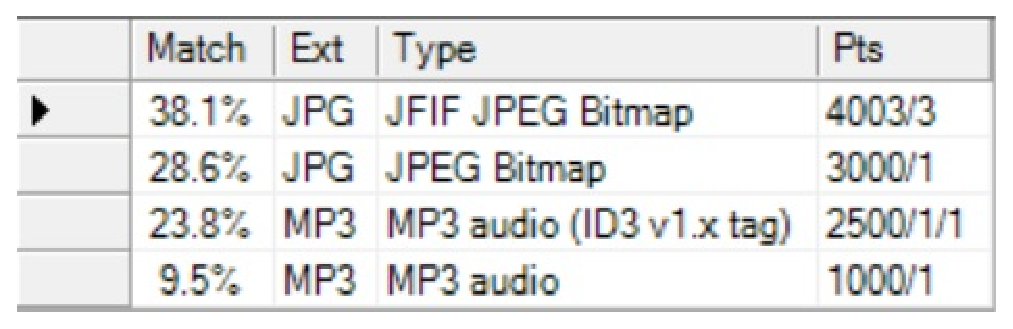
\includegraphics[width=0.5\textwidth]{01}
\end{figure}
\begin{figure}[!ht]
        \centering
        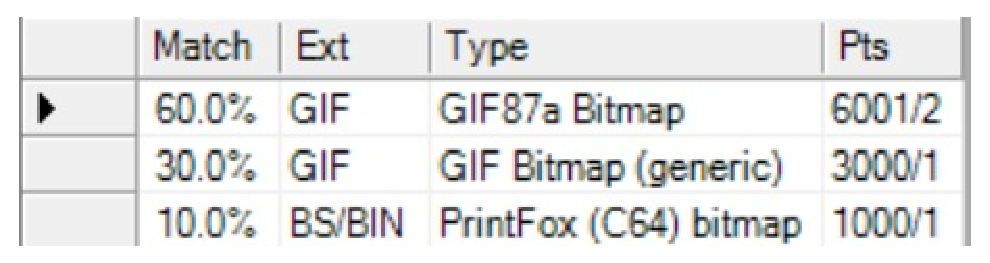
\includegraphics[width=0.5\textwidth]{02}
        \caption{File 02}
\end{figure}
\begin{figure}[!ht]
        \centering
        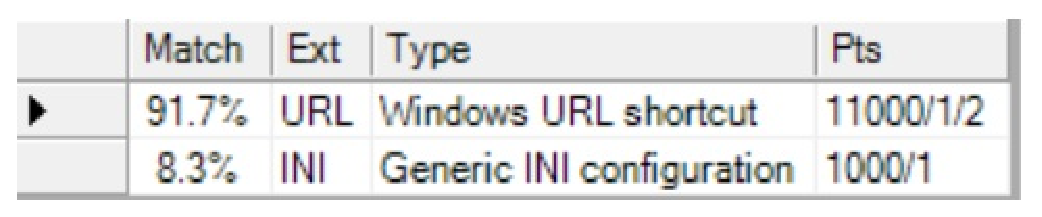
\includegraphics[width=0.5\textwidth]{03}
        \caption{File 03}
\end{figure}
\begin{figure}[!ht]
        \centering
        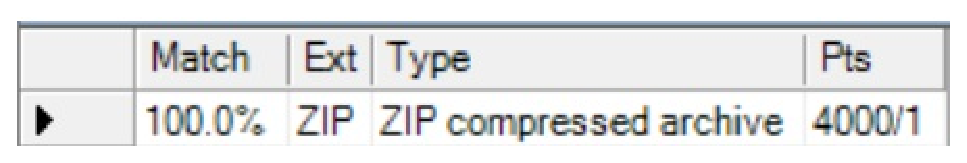
\includegraphics[width=0.5\textwidth]{04}
        \caption{File 04}
\end{figure}
\begin{figure}[!ht]
        \centering
        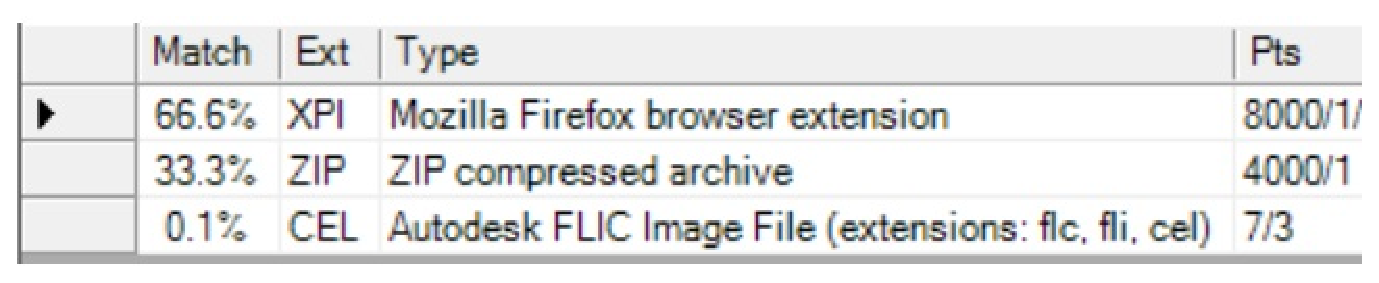
\includegraphics[width=0.5\textwidth]{05}
        \caption{File 05}
\end{figure}
\begin{figure}[!ht]
        \centering
        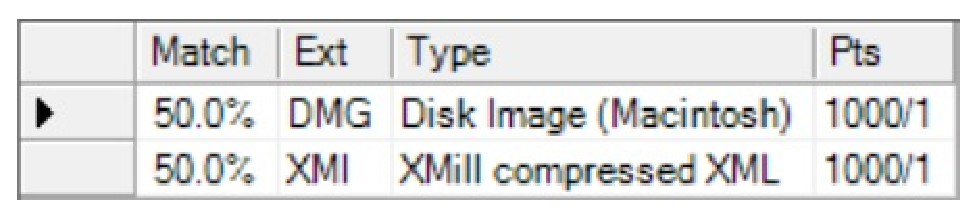
\includegraphics[width=0.5\textwidth]{06}
        \caption{File 06}
\end{figure}
\begin{figure}[!ht]
        \centering
        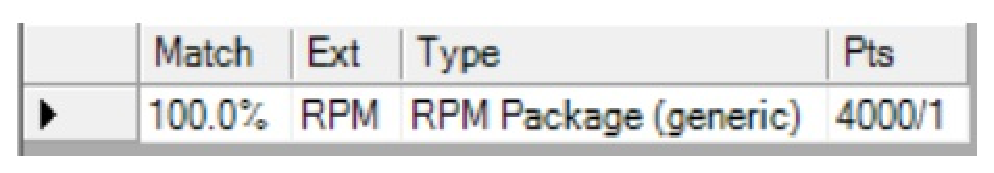
\includegraphics[width=0.5\textwidth]{07}
        \caption{File 07}
\end{figure}
\begin{figure}[!ht]
        \centering
        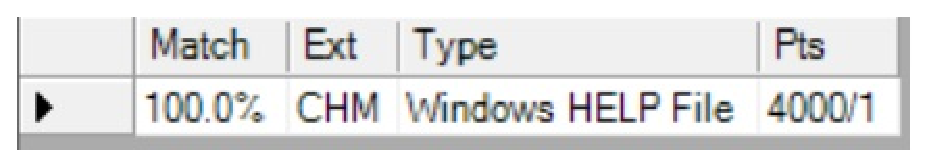
\includegraphics[width=0.5\textwidth]{08}
        \caption{File 08}
\end{figure}
\begin{figure}[!ht]
        \centering
        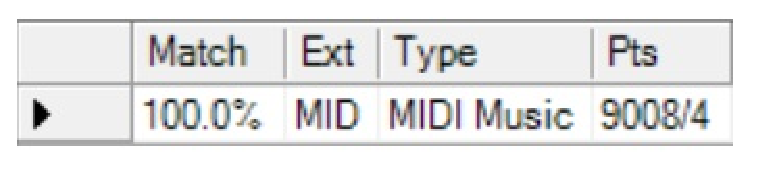
\includegraphics[width=0.5\textwidth]{09}
        \caption{File 09}
\end{figure}
\begin{figure}[!ht]
        \centering
        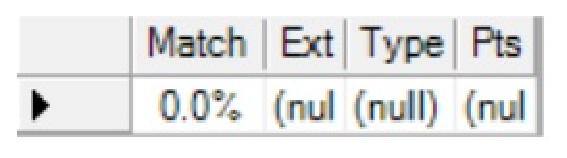
\includegraphics[width=0.5\textwidth]{10}
        \caption{File 10}
\end{figure}
\begin{figure}[!ht]
        \centering
        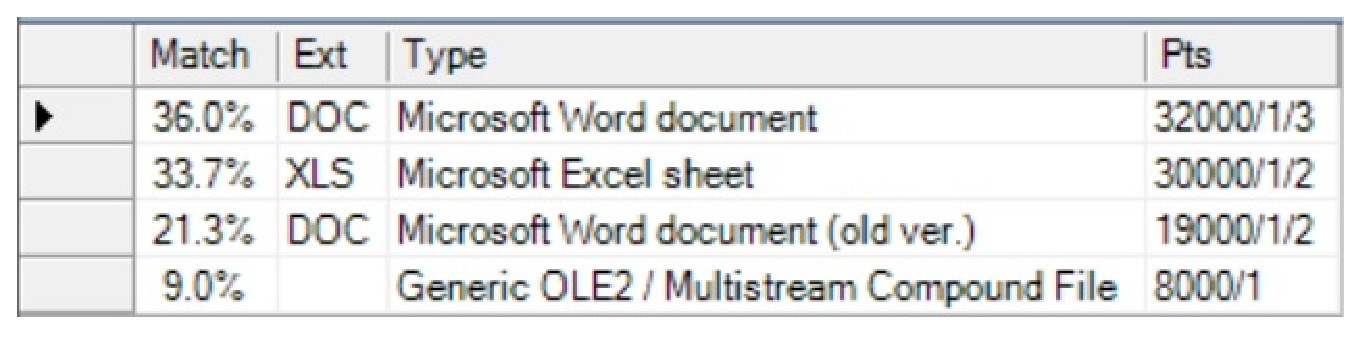
\includegraphics[width=0.5\textwidth]{11}
        \caption{File 11}
\end{figure}
\begin{figure}[!ht]
        \centering
        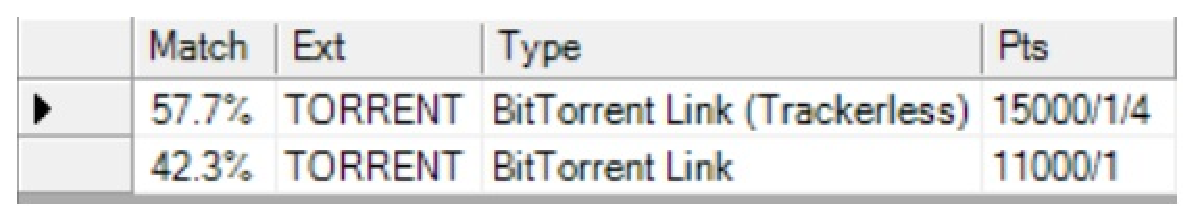
\includegraphics[width=0.5\textwidth]{12}
        \caption{File 12}
\end{figure}


\subsection{Conclusion}
After identifying the file types with the three tools mentioned above, the files where opened with the corresponding program for further examination.
The following table presents the conclusion of the findings:
\begin{center}
        \begin{tabular}{|l|p{10cm}|}
                \hline
                \textbf{File} & \textbf{Description} \\ \hline
                01 & JPEG image of a hangar filled with airplanes \\ \hline
                02 & GIF image of a generator or a motor\\ \hline
                03 & A windows shortcut for URL address containing \url{http://www.dc3.mil/challenge} \\ \hline
                04 & ZIP archive containing the tool EXIF.exe and documentation \\ \hline
                05 & ZIP archive containing Chrome plugin and install files \\ \hline
                06 & ZLIb archive - unknown contents \\ \hline
                07 & Red hat package manager archive \\ \hline
                08 & Nvidia control panel help file \\ \hline
                09 & MIDI file with the song Carmina Burana - O Fortuna \\ \hline
                10 & README file about Microsoft Check File Integrity Verifier \\ \hline
                11 & OLE file with a README about the tool Robocopy \\ \hline
                12 & .torrent file for Ubuntu ISO (AMD64 version) \\ \hline
        \end{tabular}
\end{center}
%----------------------------------------------------
%-------------- EXERCISE 3
%----------------------------------------------------
\newpage
\section{Exercise 3: Anti Files Forensics}
Inside the folder Exercise3\textunderscore Anti\textunderscore Files\textunderscore Forensics. Two files named 'c.mp3' and 'Suspicious\textunderscore file' where present. The hash sums for both files are listed below:
\begin{lstlisting}[caption=SHA256 and MD5 sum of files in folder]
sha256sum *
83a15326cf9066a36defbe4f8a0633ec16867999c5910257807493ce250a3548  c.mp3
cec6534e8ddc4f5f9e9b2a0cedb438a8419a5ffd08ecfe059467630f624d5b1a  Suspicious_File

md5sum *
670a8c0db494ced4882b44b27dbd6af2  c.mp3
63017bb2a213fa440191b204929ab0f7  Suspicious_File
\end{lstlisting}
More information about the files could be obtained by using the file command:

\begin{lstlisting}[caption=Result from 'file' command]
c.mp3: Audio file with ID3 version 2.255.216, unsynchronized frames, extended header, experimental, footer present

Suspicious_File: Composite Document File V2 Document, Cannot read section info
\end{lstlisting}

\subsection{Foremost}
Using the Linux tool foremost\footnote{\url{https://en.wikipedia.org/wiki/Foremost_(software)}} it was discovered that the files contained other content than the file ending indicated.

\subsubsection{c.mp3}
Using foremost on the file 'c.mp3' one additional .jpg file were found.
\begin{lstlisting}[caption= foremost file 'c']
foremost c.mp3 -v -o c

Foremost version 1.5.7 by Jesse Kornblum, Kris Kendall, and Nick Mikus
Audit File

Foremost started at Sun Sep 24 16:11:49 2017
Invocation: foremost c.mp3 -v -o c
Output directory: /home/fluchey/Documents/Skola/DIFO/Lab1/Exercise3_Anti_Files_Forensics/c
Configuration file: /etc/foremost.conf
Processing: c.mp3
|------------------------------------------------------------------
File: c.mp3
Start: Sun Sep 24 16:11:49 2017
Length: 18 KB (19332 bytes)

Num      Name (bs=512)         Size      File Offset     Comment

0:      00000000.jpg          18 KB               3
*|
Finish: Sun Sep 24 16:11:49 2017

1 FILES EXTRACTED

jpg:= 1 # Here we can see that one additional .jpg file were extracted
------------------------------------------------------------------

Foremost finished at Sun Sep 24 16:11:49 2017
\end{lstlisting}

Further examination of the extracted file showed that it was an image of the Actress Keira Knightley\footnote{\url{http://www.imdb.com/name/nm0461136/}} and the file was named '00000000.jpg'.
\begin{figure}[ht]
        \centering
        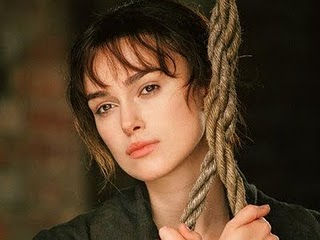
\includegraphics[width=0.5\textwidth]{00000000.jpg}
        \caption{Extracted picture from 'c.mp3'}
\end{figure}





\subsubsection{Suspicious\textunderscore File}



Using foremost on the file 'Suspicious\textunderscore File' one additional .ole\footnote{\url{https://en.wikipedia.org/wiki/Object_Linking_and_Embedding}} file were found

\begin{lstlisting}[caption= foremost file 'Suspicious\textunderscore File']
foremost Suspicious_File -v -o sus
Foremost version 1.5.7 by Jesse Kornblum, Kris Kendall, and Nick Mikus
Audit File

Foremost started at Sun Sep 24 16:19:26 2017
Invocation: foremost Suspicious_File -v -o sus
Output directory: /home/fluchey/Documents/Skola/DIFO/Lab1/Exercise3_Anti_Files_Forensics/sus
Configuration file: /etc/foremost.conf
Processing: Suspicious_File
|------------------------------------------------------------------
File: Suspicious_File
Start: Sun Sep 24 16:19:26 2017
Length: 1 MB (1304576 bytes)

Num      Name (bs=512)         Size      File Offset     Comment

0:      00000000.ole          12 KB               0
*|
Finish: Sun Sep 24 16:19:26 2017

1 FILES EXTRACTED

ole:= 1 # Here we can see that on .ole file were extracted
------------------------------------------------------------------

Foremost finished at Sun Sep 24 16:19:26 2017
\end{lstlisting}
The extracted .ole file failed to open in any recommended software. Both 'Suspicious\textunderscore File' and the extracted .ole file were submitted to malware scanning site Cryptam\footnote{\url{https://www.cryptam.com/}}.
Cryptam discovered that 'Suspicious\textunderscore File' contained an embedded executable.

\begin{figure}[ht]
        \centering
        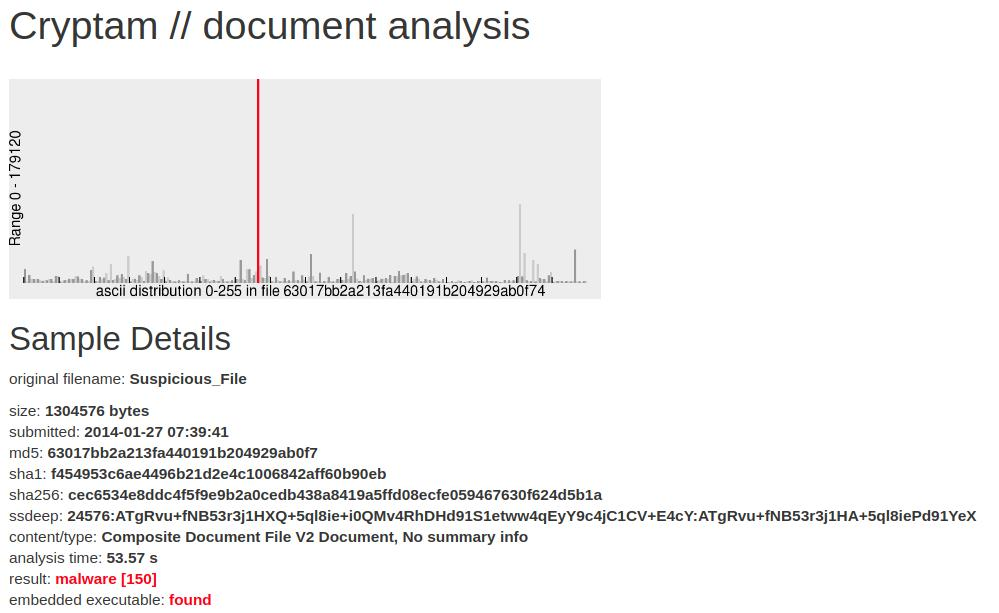
\includegraphics[width=\textwidth]{cryptam_sus}
        \caption{Cryptam result of 'Suspicious\textunderscore File'}
\end{figure}

And it found the .ole file to be suspicious

\begin{figure}[ht]
  \centering
  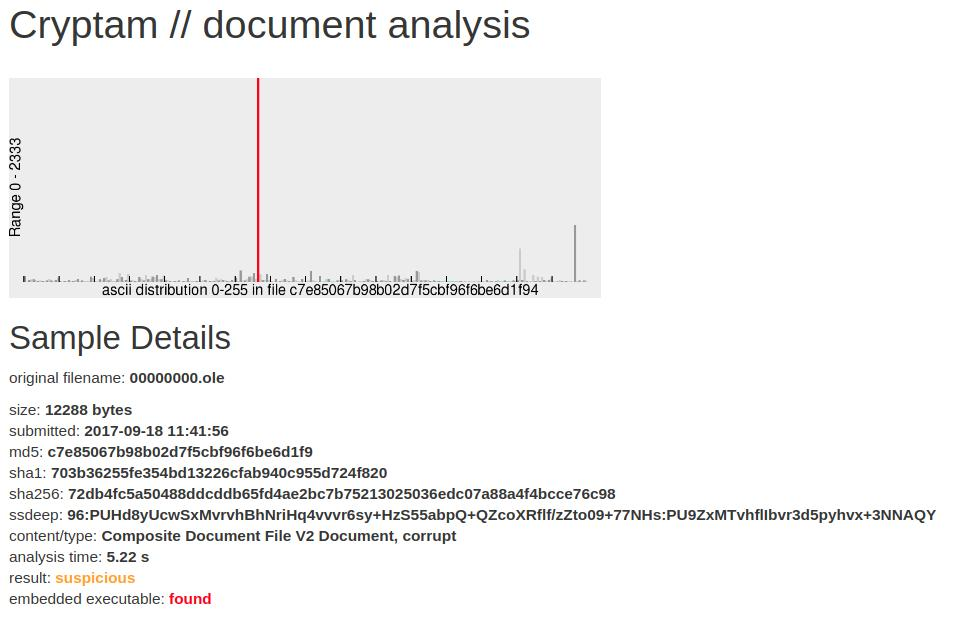
\includegraphics[width=\textwidth]{images/cryptam_ole}
  \caption{Cryptam result of '00000000.ole'}
\end{figure}




%----------------------------------------------------
%-------------- EXERCISE 4
%----------------------------------------------------
\newpage
\section{Exercise 4: Acquisition}
%----------------------------------------------------
%-------------- EXERCISE 5
%----------------------------------------------------
\newpage
\section{Exercise 5: Cracking }
%----------------------------------------------------
%-------------- EXERCISE 6
%----------------------------------------------------
\newpage
\section{Exercise 6 - Steganography}
in the folder Exercise6\textunderscore Steganography two files named 'c1l.png' and 'c2l.png' were present.

\begin{lstlisting}[caption= SHA256 and MD5 sum of files in Exercise6\textunderscore Steganography]
sha256sum *
d8ad7abb90ee967108f37d3b702016827219692e25fc840fb7e737ba0b7eab00  c1l.png
822e27042277d9588d699adcf1f3da7428cad7de9506eda7ae3644f858574e1f  c2l.png

md5sum *
601450fd443b42f4ece0e3f001ed73b3  c1l.png
b914cc2043a6d5b31ff4bb6f5f1291fc  c2l.png
\end{lstlisting}

The file ending '.png' indicate that the files are images. Opening them in an image viewing program confirms that they are in fact images.

\begin{figure}[ht]
  
\includegraphics[width=\textwidth]{images/c1l}
  \caption{Image of 'c1l.png'}
  \centering
\end{figure}





\begin{figure}[ht]
  
\includegraphics[width=\textwidth]{images/c2l}
  \caption{Image of 'c2l.png'}
  \centering
\end{figure}

The files were opened in a Hex Editor (\textbf{Bless}) to visually examine them. Nothing out of the ordinary was found for either file.
The files were also opened in \textbf{pngcheck} and the following was reported:


\begin{lstlisting}[caption=c1l.png]
No errors detected in c1l.png (7 chunks, 92.7% compression).
\end{lstlisting}

\begin{lstlisting}[caption=c2l.png]
No errors detected in c2l.png (3 chunks, 92.7% compression).
\end{lstlisting}

Opening the files in the program \textbf{stepic} with the command:

\begin{lstlisting}[caption=stepic command]

stepic -d -i ~/Desktop/Lab1/Exercise6_Steganography/c1l.png -o c1lout

stepic -d -i ~/Desktop/Lab1/Exercise6_Steganography/c2l.png -o c2lout

\end{lstlisting}

Reveals the following information:\\

\underline{Output for c1l.png, contains:}\\The text \textbackslash FF (while viewed in Linux/Mac OS)
xFF (while viewed through Notepad++ in Windows)

Different character sets were tried to see if the text could be understood.\\


\underline{Output for c2l.png, contains:}\\ \url{http://xdsa5xcrrrxxxolc.onion/}

Which is an address for the TOR network, an adress for an online pharmacy.


To find out more information about the two files and to find if there was any more hidden messages, a comparation of the two files were performed with the command:\\

\begin{lstlisting}
compare c1l.png c2l.png compareresult.png
\end{lstlisting}

Which produces a new image containing the result of the the image comparation. I.e. the resulting differences between the two files.

\begin{figure}[ht]
	
\includegraphics[width=\textwidth]{images/compareresult.png}
	\caption{Image of 'compareresult.png'}
	\centering
\end{figure}

The red portion shows a detected difference between the two files. There are differences between the two files and it is contained in the red highlighted portion in the above image.

The files were also examined by ExifTool\footnote{\url{https://en.wikipedia.org/wiki/ExifTool}}. The output from
ExifTool differed and som information were not present in 'c2l.png'

\begin{lstlisting}[caption=ExifTool output for 'c1l.png']
exiftool c1l.png
ExifTool Version Number         : 10.60
File Name                       : c1l.png
Directory                       : .
File Size                       : 18 kB
File Modification Date/Time     : 2017:08:09 16:36:22+02:00
File Access Date/Time           : 2017:09:28 10:34:39+02:00
File Inode Change Date/Time     : 2017:09:15 12:24:53+02:00
File Permissions                : rwxr-xr-x
File Type                       : PNG
File Type Extension             : png
MIME Type                       : image/png
Image Width                     : 403
Image Height                    : 157
Bit Depth                       : 8
Color Type                      : RGB with Alpha
Compression                     : Deflate/Inflate
Filter                          : Adaptive
Interlace                       : Noninterlaced
Significant Bits                : 8 8 8 8         # // These rows are not
Pixels Per Unit X               : 7500            # // on the
Pixels Per Unit Y               : 7500            # // output for
Pixel Units                     : meters          # // c2l.png
Image Size                      : 403x157
Megapixels                      : 0.063
\end{lstlisting}

\begin{lstlisting}[caption=ExifTool output for 'c2l.png']
exiftool c2l.png
ExifTool Version Number         : 10.60
File Name                       : c2l.png
Directory                       : .
File Size                       : 18 kB
File Modification Date/Time     : 2017:08:09 16:40:16+02:00
File Access Date/Time           : 2017:09:28 10:36:15+02:00
File Inode Change Date/Time     : 2017:09:15 12:24:53+02:00
File Permissions                : rwxr-xr-x
File Type                       : PNG
File Type Extension             : png
MIME Type                       : image/png
Image Width                     : 403
Image Height                    : 157
Bit Depth                       : 8
Color Type                      : RGB with Alpha
Compression                     : Deflate/Inflate
Filter                          : Adaptive
Interlace                       : Noninterlaced
Image Size                      : 403x157
Megapixels                      : 0.063
\end{lstlisting}
The files were further examined by the tool StegSolve \footnote{\url{http://www.caesum.com/handbook/Stegsolve.jar}} but no further findings were found.


This leads us to the conclusion that cl1.png is the original and that c2l.png is the only image containing a steganographic hidden message.



%\bibliographystyle{plain}
%\bibliography{bibtex}
%\bibdata{bibtex}

\end{document}
